
\chapter{Podstawy teoretyczne}

coś tutaj można napisać z~3-4 liniki wprowadzenia co to za rozdział, we wstępie to jest opisane
 
\section{System oznaczania zębów}

Istnieje wiele systemów służących do zapisywania stanu uzębienia pacjentów. Pomagają one w~przejrzysty sposób przechowywać dane, które mogą być przekazywane między pracownikami służby zdrowia wykorzystującymi różne programy oraz standardy. Nie wymagają wówczas skomplikowanej analizy - jednoznacznie i~w~prosty sposób przedstawiają wprowadzone wcześniej dane. Dodatkowo są~zrozumiałe i~przystępne dla pacjentów.

Każdy z~systemów wyróżnia zbiór reguł, według których zęby, z~rozróżnieniem na zęby mleczne oraz stałe, są kolejno nazywane. W~najbardziej popularnych systemach, które zostały przedstawione poniżej, zęby podzielone są na cztery podzbiory oznaczane jako: łuk górny prawy, łuk górny lewy, łuk dolny lewy oraz łuk dolny prawy. Schematy przedstawiają na planie krzyża uzębienie widziane z~perspektywy lekarza, a~nazwy dotyczą perspektywy pacjenta.

\subsection{Przegląd systemów}
\subsubsection{System łaciński}

\renewcommand*{\tablename}{Schemat}

System ten wykorzystuje w~nazewnictwie pierwsze litery łacińskich nazw zębów. Stąd w~każdej ćwiartce dwa siekacze oznaczane są literą \textit{I} - od słowa \textit{incisivi} - i~kolejno numerowane, kły literą \textit{C} - od słowa \textit{canini}, oznaczenie dwóch przedtrzonowców pochodzi od słowa \textit{premolares} - litera \textit{P} oraz trzech trzonowców od słowa \textit{molares} - litera \textit{M}. W~systemie łacińskim oprócz nazwy zęba, która powtarza się w~czterech podzbiorach, dodaje się także nazwę ćwiartki, do której ząb należy, definiując czy jest górna czy też dolna oraz czy lewa albo prawa.\\

\begin{table}[h t]
\centering
\begin{tabular}{c c c c c c c c c | c c c c c c c c c}
M\textsubscript{3} & M\textsubscript{2} & M\textsubscript{1} & P\textsubscript{2} & P\textsubscript{1} & C & I\textsubscript{2} & I\textsubscript{1} &&& I\textsubscript{1} & I\textsubscript{2} & C & P\textsubscript{1} & P\textsubscript{2} & M\textsubscript{1} & M\textsubscript{2} & M\textsubscript{3}
\\ [1ex] \hline \rule{0pt}{1.2\normalbaselineskip}
M\textsubscript{3} & M\textsubscript{2} & M\textsubscript{1} & P\textsubscript{2} & P\textsubscript{1} & C & I\textsubscript{2} & I\textsubscript{1} &&& I\textsubscript{1} & I\textsubscript{2} & C & P\textsubscript{1} & P\textsubscript{2} & M\textsubscript{1} & M\textsubscript{2} & M\textsubscript{3}
\end{tabular}
\caption{\label{tab:tab1} System łaciński: zęby stałe}
\end{table}

Opisane powyżej nazewnictwo dotyczy zębów stałych człowieka. Zęby mleczne oznacza się jednak analogicznie, zamieniając jedynie wielkie litery na małe - \textit{i}, \textit{c}, \textit{m} oraz opisując pięć zębów w~każdej ćwiartce - dwa siekacze, kieł oraz dwa zęby trzonowe.

\begin{table}[h t]
\centering
\begin{tabular}{c c c c c c | c c c c c c}
m\textsubscript{2} & m\textsubscript{1} & c & i\textsubscript{2} & i\textsubscript{1} &&& i\textsubscript{1} & i\textsubscript{2} & c & m\textsubscript{1} & m\textsubscript{2}
\\ [1ex] \hline \rule{0pt}{1.2\normalbaselineskip}
m\textsubscript{2} & m\textsubscript{1} & c & i\textsubscript{2} & i\textsubscript{1} &&& i\textsubscript{1} & i\textsubscript{2} & c & m\textsubscript{1} & m\textsubscript{2}
\end{tabular}
\caption{\label{tab:tab2} System łaciński: zęby mleczne}
\end{table}

\subsubsection{System Zsigmondy’ego}

System Zsigmondy'ego, podobnie jak system łaciński, definiuje taką samą nazwę dla odpowiadających sobie zębów w~kolejnych ćwiartkach i~dodaje do niej oznaczenie jednej z~czterech części. Zęby są tutaj numerowane od 1 do 8, zaczynając od siekaczy znajdujących się najbliżej środka krzyża na schemacie, kończąc na ostatnim trzonowcu. Do numeru dodaje się symbol odpowiadający kątowi prostemu fragmentu krzyża danej ćwiartki. Zgodnie z~tymi zasadami drugi lewy górny siekacz oznacza się symbolami \cfbox[lb]{black}{2}, a~prawy dolny pierwszy trzonowiec symbolami \cfbox[tr]{black}{6}.\\

\begin{table}[h t]
\centering
\begin{tabular}{c c c c c c c c c | c c c c c c c c c}
8 & 7 & 6 & 5 & 4 & 3 & 2 & 1 &&& 1 & 2 & 3 & 4 & 5 & 6 & 7 & 8
\\ [1ex] \hline \rule{0pt}{1.2\normalbaselineskip}
8 & 7 & 6 & 5 & 4 & 3 & 2 & 1 &&& 1 & 2 & 3 & 4 & 5 & 6 & 7 & 8
\end{tabular}
\caption{\label{tab:tab3} System Zsigmondy’ego: zęby stałe}
\end{table}

Zęby mleczne w~tym systemie oznacza się analogicznie, zamieniając jedynie cyfry arabskie na rzymskie.

\begin{table}[h t]
\centering
\begin{tabular}{c c c c c c | c c c c c c}
V & IV & III & II & I &&& I & II & III & IV & V
\\ [1ex] \hline \rule{0pt}{1.2\normalbaselineskip}
V & IV & III & II & I &&& I & II & III & IV & V
\end{tabular}
\caption{\label{tab:tab4} System Zsigmondy’ego: zęby mleczne}
\end{table}

System Zsigmondy'ego jest dużo łatwiejszy w~użyciu w~porównaniu z~systemem łacińskim. Pozwala na znacznie szybszy zapis i~odczyt danych, gdyż nie wymaga długiego opisu każdej ćwiartki. Jego wadą jest użycie symboli, których nie można łatwo wprowadzać do systemów komputerowych przy użyciu klawiatury. Powstały jednak zamienniki, których można używać. Na przykład opis \cfbox[tr]{black}{6}~jest równoznaczny opisowi 6\textbackslash{}, wykorzystującemu symbol \textit{backslask}, a~oznaczenie \cfbox[lb]{black}{2} równoznaczne oznaczeniu \textbackslash2. Analogicznie wykorzystuje się znak \textit{slash} dla ćwiartek górnej prawej oraz dolnej lewej.

\subsubsection{System Haderupa}

System Haderupa, bardzo popularny w~Skandynawii, jest systemem, w~którym zęby stałe numeruje się tak samo jak w~systemie Zsigmondy’ego. Różni się jedynie zasadą, która określa wybraną ćwiartkę. Zęby łuku górnego oznacza się tutaj plusami, a~łuku dolnego minusami. Z kolei prawą i~lewą stronę odróżnia się na podstawie położenia znaku + lub -. Zęby prawych łuków oznacza się najpierw cyfrą, a~później odpowiednim znakiem, a~zęby łuków lewych odwrotnie - najpierw znakiem, a~później liczbą.\\

\begin{table}[h t]
\centering
\begin{tabular}{c c c c c c c c c | c c c c c c c c c}
8+ & 7+ & 6+ & 5+ & 4+ & 3+ & 2+ & 1+ &&& +1 & +2 & +3 & +4 & +5 & +6 & +7 & +8
\\ [1ex] \hline \rule{0pt}{1.2\normalbaselineskip}
8- & 7- & 6- & 5- & 4- & 3- & 2- & 1- &&& -1 & -2 & -3 & -4 & -5 & -6 & -7 & -8
\end{tabular}
\caption{\label{tab:tab5} System Haderupa: zęby stałe}
\end{table}

Aby odróżnić zęby mleczne od stałych przed każdą cyfrą dodaje się cyfrę 0. Pozostałe oznaczenia, znaki plusów i~minusów, dodaje się na podstawie zasad omówionych dla zębów stałych.\\

\begin{table}[h t]
\centering
\begin{tabular}{c c c c c c | c c c c c c}
05+ & 04+ & 03+ & 02+ & 01+ &&& +01 & +02 & +03 & +04 & +05 \\
[1ex] \hline \rule{0pt}{1.2\normalbaselineskip}
05- & 04- & 03- & 02- & 01- &&& -01 & -02 & -03 & -04 & -05
\end{tabular}
\caption{\label{tab:tab6} System Haderupa: zęby mleczne}
\end{table}

System Haderupa, oprócz krótszego zapisu, który odróżnia go od systemu łacińskiego, wyróżnia się łatwością wprowadzania danych, gdyż symbole, które wykorzystuje można z~łatwością wprowadzać do systemów komputerowych używając klawiatury. Znaki plusa oraz minusa, a~także dodatkowego zera na początku oznaczenia mogą jednak powodować problemy. Programy komputerowe zapis \textit{05} traktują jako \textit{5}, a~plusy i~minusy jako działania na tych liczbach.

\subsubsection{System Viohla}

System Viohla, nazywany także systemem międzynarodowym, jest najbardziej rozpowszechnionym systemem oznaczania zębów. Od roku 1970 jest oficjalnie uznawany jako norma ISO-3950, która jest zalecana przez WHO. System ten charakteryzuje się łatwością zapisu danych, a~także prostotą ich werbalnego przekazu.

Kolejne zęby, zarówno zęby stałe jak i~mleczne, w~systemie Viohla oznaczane są dwoma cyframi. Pierwsza cyfra oznacza numer ćwiartki, do której ząb należy, a~druga numer zęba w~tej ćwiartce, licząc od środka łuku zębowego. Ćwiartki numerowane są rozpoczynając zawsze od górnego prawego łuku zgodnie z~ruchem wskazówek zegara. Dla zębów stałych przyjmują one numery z~zakresu 1 - 4, a~dla zębów mlecznych z~zakresu 5 - 8.\\

\begin{table}[h t]
\centering
\begin{tabular}{c c c c c c c c c | c c c c c c c c c}
18 & 17 & 16 & 15 & 14 & 13 & 12 & 11 &&& 21 & 22 & 23 & 24 & 25 & 26 & 27 & 28
\\ [1ex] \hline \rule{0pt}{1.2\normalbaselineskip}
48 & 47 & 46 & 45 & 44 & 43 & 42 & 41 &&& 31 & 32 & 33 & 34 & 35 & 36 & 37 & 38
\end{tabular}
\caption{\label{tab:tab7} System Viohla: zęby stałe}
\end{table}

\begin{table}[h t]
\centering
\begin{tabular}{c c c c c c | c c c c c c}
55 & 54 & 53 & 52 & 51 &&& 61 & 62 & 63 & 64 & 65
\\ [1ex] \hline \rule{0pt}{1.2\normalbaselineskip}
85 & 84 & 83 & 82 & 81 &&& 71 & 72 & 73 & 74 & 75
\end{tabular}
\caption{\label{tab:tab8} System Viohla: zęby mleczne}
\end{table}

\subsubsection{System uniwersalny}

System uniwersalny nieco różni się od systemów opisanych powyżej. Jako jedyny z~wymienionych nie uwzględnia w~swoich oznaczeniach poszczególnych ćwiartek. Zęby w~tym systemie numerowane są kolejnymi liczbami naturalnymi. Łuk górny numerowany jest rozpoczynając od ostatniego trzonowca prawego, aż do ostatniego trzonowca lewego, a~łuk dolny odwrotnie - od ostatniego trzonowca lewego, aż do ostatniego prawego.\\

\begin{table}[h t]
\centering
\begin{tabular}{c c c c c c c c c | c c c c c c c c c}
1 & 2 & 3 & 4 & 5 & 6 & 7 & 8 &&& 9 & 10 & 11 & 12 & 13 & 14 & 15 & 16
\\ [1ex] \hline \rule{0pt}{1.2\normalbaselineskip}
32 & 31 & 30 & 29 & 28 & 27 & 26 & 25 &&& 24 & 23 & 22 & 21 & 20 & 19 & 18 & 17
\end{tabular}
\caption{\label{tab:tab9} System uniwersalny: zęby stałe}
\end{table}

Zęby mleczne nazywane są analogicznie. W~tej samej kolejności zębom przypisuje się kolejne wielkie litery alfabetu.\\

\begin{table}[h t]
\centering
\begin{tabular}{c c c c c c | c c c c c c}
A & B & C & D & E &&& F & G & H & I & J
\\ [1ex] \hline \rule{0pt}{1.2\normalbaselineskip}
T & S & R & Q & P &&& O & N & M & L & K
\end{tabular}
\caption{\label{tab:tab10} System uniwersalny: zęby mleczne}
\end{table}

System w~prosty sposób jednoznacznie definiuje kolejne zęby łuków. Jego dużą wadą jest jednak konieczność pamiętania wszystkich kolejnych numerów, które nie wskazują bezpośrednio na żadną ćwiartkę, więc nie pozwalają na szybkie i~intuicyjne określenie położenia wskazanego zęba.

\renewcommand*{\tablename}{Tabela}

\subsection{Wybór systemu}

Implementowany w~ramach pracy inżynierskiej diagram zębowy opiera się o~system Viohla. System ten jest powszechnie używanym systemem, dlatego zdaje się być zrozumiały dla większości stomatologów i~ich asystentów - docelowych użytkowników aplikacji. Dodatkowo jest on bardzo wygodny w~implementacji. Program nie musi przechowywać dodatkowych oznaczeń dla poszczególnych zębów, a~jedynie indeksować je, wykorzystując kolejne ich numery. Nie występują tutaj także problemy z~błędnie pomijanymi zerami, czy też plusami i~minusami, jak w~systemie Haderupa.



\subsection{Nazewnictwo zębów}
Powyżej opisane systemy pozwalają na przedstawianie diagramów zębowych z~rozróżnieniem na poszczególne zęby - 32 zęby stałe oraz 20 zębów mlecznych. Dokumentacja stomatologiczna musi być jednak znacznie bardziej szczegółowa i~opisywać poszczególne części kolejnych zębów. Stąd w~opisach stanu uzębienia pacjentów wyróżnia się pięć osobnych powierzchni, które w~literaturze mają przypisane odpowiednie nazwy.\cite{teethAnatomy} Wyróżnia się:

\begin{itemize}
    \item powierzchnię wargową lub policzkową - zewnętrzną powierzchnię łuku zębowego,
    \item powierzchnię językową - wewnętrzną powierzchnię łuku zębowego,
    \item powierzchnię zgryzową/okluzyjną lub brzeg sieczny - powierzchnię stykającą się z~zębami przeciwnego łuku zębowego,
    \item dwie powierzchnie styczne - bliższą (mezjalną) oraz dalszą (dystalną) - powierzchnie stykające się odpowiednio z~mniej lub bardziej oddalonym od środka łuku zębem sąsiadującym w~ramach tej samej ćwiartki.
\end{itemize}



\subsection{Choroby zębów}
Diagramy zębowe służą przechowywaniu informacji na temat chorób poszczególnych zębów. Istnieje wiele stanów, w~których zęby mogą się znaleźć. Zalicza się do nich wypełnienie, próchnicę, ubytki, implanty, także informację o~braku zęba, który jeszcze nie jest wyrżnięty lub został usunięty.\cite{teethDiseases} Różne diagramy w~różnym stopniu precyzują poszczególne zmiany, dzieląc je na bardziej szczegółowe lub grupując podobne.

\begin{itemize}
    \item Jakie są choroby zębów
    \item każdą z~chorób opisać po 3-4 linijki
    \item można się rozpisać trochę o~próchnicy bo powinno to być proste, powinno być dużo na stronach popularno naukowych
\end{itemize}

\subsection{Rozpoznawanie mowy}
Rozpoznawanie mowy, szczególnie w~języku polskim, jest trudnym zadaniem.\cite{cloudSpeechAPI} W~celu stworzenia interfejsu głosowego do diagramu zębowego, użyto Google Speech Recognition API.

System rozpoznawania, stworzony przez firmę Google, używa trzech osobnych modeli:
\begin{itemize}
    \item Model akustyczny
    \item Model wymowy
    \item Model językowy
\end{itemize}
Każdy z~modeli jest trenowany osobno. Aczkolwiek ostatecznie są one skomponowane w~jeden duży graf wyszukiwania. W~ogólności działanie systemu jest następujące. Do system zostaje wprowadzony plik audio, czyli przebieg fali dźwiękowej, w~określonym języku. Przebieg zostaje przepuszczony przez graf wyszukiwania. Podczas przechodzenia grafu, szukana jest ścieżka najmniejszego oporu - to znaczy znalezienie takiej sekwencji słów, która ma największe prawdopodobieństwo.

Model akustyczny identyfikuje fonemy, które najprawdopodobniej występują w~próbce audio. Pobiera przebieg, dzieli go na małe segmenty czasowe, wdraża analizę częstotliwości i~generuje rozkład prawdopodobieństwa na wszystkie stany fonemów, dla tego konkretnego wejścia. Wektor częstotliwości fali, dopasowany do rozkładu prawdopodobieństwa, identyfikuje w~ten sposób, które fonemy z~większym prawdopodobieństwem niż inne znajdują się w~tej próbce dźwięku. Dostarczając w~ten sposób sekwencję fonemów, które istnieją w~tym wejściu w~czasie.

Następnie zaczyna działać model wymowy. Pobiera rozkłady prawdopodobieństwa fonemów z~modelu akustycznego, porównuje je z~obszernym leksykonem definiującym prawidłowe sekwencje fonemów dla słów określonego języka i~ogranicza możliwe sekwencje fonemów do tych, które mają sensu w~tym języku.

Łącząc modele akustyczne i~wymowy, mamy system gdzie wejściem jest dźwięk, a~wyjściem są słowa. W~celu zapewnienia niezawodnego wyszukiwania głosowego, należy znaleźć istnieją kombinacje słów, które są bardziej prawdopodobne niż inne. Model językowy oblicza częstotliwości wszystkich sekwencji słów od jednego do pięciu słów. Tym samym ogranicza możliwe sekwencje słów, które można utworzyć z~dwóch wyżej wymienionych modeli, do tych, które są rozsądnymi kombinacjami w~danym języku. Ostateczny algorytm wyszukiwania wybierze następnie sekwencję słów, która ma najwyższą częstotliwość występowania w~danym języku.


\section{Analiza odchylenia toru odwodzenia żuchwy}
z rzeczy które wydaje mi się że można opisać:
\begin{itemize}
    \item przykłady rozpoznawania innych części ciała (aktualny state-of-the-art) + obrazki (to można też pokazać w~technologiach odnośnie konkretnej biblioteki)
    \item na pewno jakieś mądre obrazki do tej teorii co już jest np. sieci neuronowej
    \item 
\end{itemize}
\subsection{Nieprawidłowość w torze odwodzenia żuchwy}



\subsection{Rozpoznawanie obrazów}
    Dziedzina rozpoznawania obrazów (ang. \emph{Computer vision}) ma na celu tworzenie obliczeniowych modeli ludzkiego narządu wzroku. Narzędzia z~wielu obszarów nauki i~inżynierii łączone są w~autonomiczne systemy zdolne do wykonywania zadań niegdyś wymagających uwagi człowieka lub zupełnie dla niego nieosiągalnych. W~dyscyplinie tej można wyróżnić liczne konkretne wyzwania:
\begin{itemize}
    \item \textbf{Detekcja obiektów i~cech} polegająca na znajdowaniu fragmentów zawierających najbardziej istotne informacje na temat zawartości obrazu. Do często rozpatrywanych cech należą m. in. krawędzie, wierzchołki, plamy (\emph{blobs}), grzbiety, a~w~przypadku video obiekty będące w~ruchu.
    \item \textbf{Identyfikacja obiektów}, czyli przypisywanie obrazów lub ich fragmentów do semantycznych klas opisujących rodzaj obiektu, bądź konkretny okaz (np. rozpoznawanie osoby po twarzy).
    \item \textbf{Śledzenie obiektów} mające na celu ustalenie położenia zadanego obszaru w~trakcie nagrania, biorąc pod uwagę takie zjawiska jak jego zakrywanie, rotacja, zmiany barwy itd. 
    \item \textbf{Przepływ optyczny (\emph{Optical flow})}, czyli rozpoznawanie ruchów każdego punktu (z dokładnością do piksela) będącego na nagraniu, w~celu oszacowania przemieszczeń powierzchni względem obserwatora.
    \item \textbf{Odtwarzanie obrazów} polegające na usuwaniu szumu oraz uzupełnianiu brakujących fragmentów, klatek. Wykorzystywane metody mogą być bardzo proste, lub wyspecjalizowane do konkretnych danych i~rodzajów zakłóceń. \cite{Szeliski2011}
\end{itemize}

\subsubsection{Główne podejścia w~rozpoznawaniu obrazów}

\begin{figure}[ht!]
\centering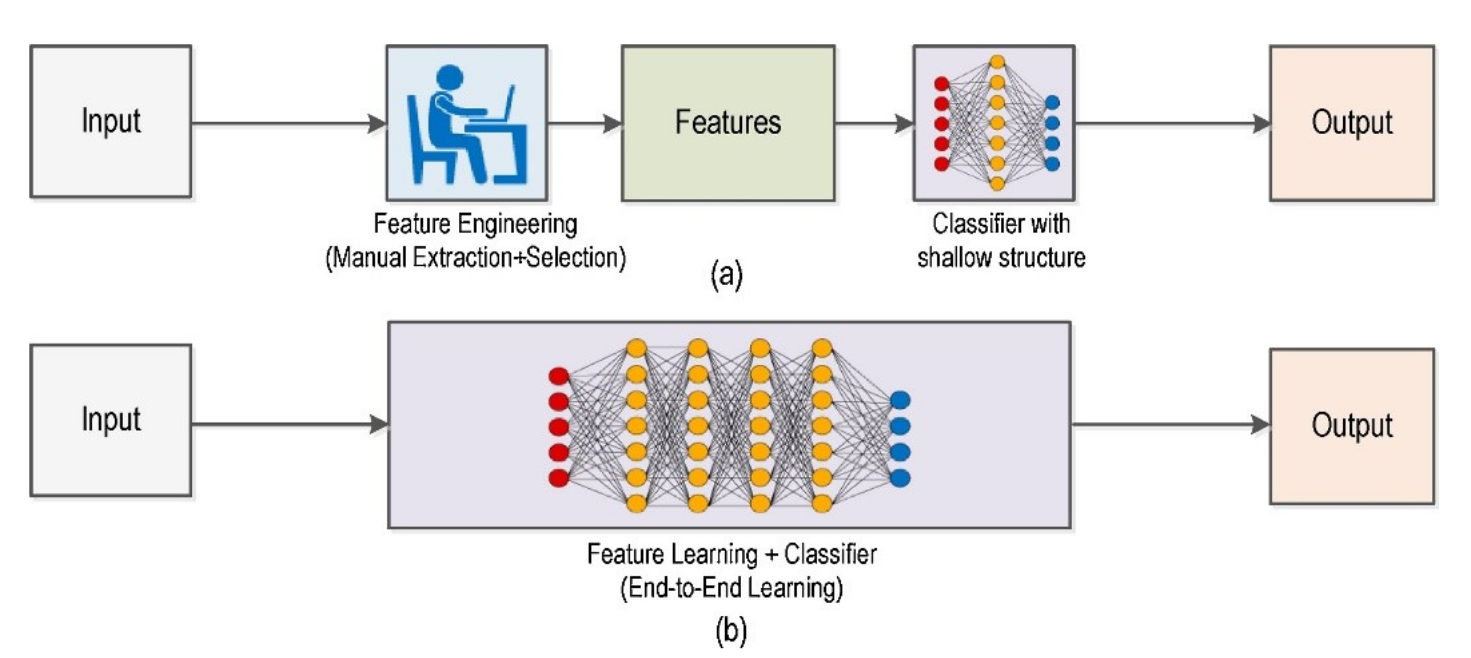
\includegraphics[width=115mm]{figures/dl_v_traditional.png}
\caption{Porównanie procesu budowania modelu rozpoznawania obrazów w~sposób deskryptywny (a) oraz za pomocą uczenia głębokiego (b) \cite{walsh19}.}
\label{fig:walsh19}
\end{figure}

Rozwój teorii sztucznych sieci neuronowych oraz technologii umożliwiających intensywne gromadzenie i~przetwarzanie danych zapoczątkowały nowe podejście w~sposobie rozwiązywania klasycznych problemów rozpoznawania obrazów. W~drugiej dekadzie XXI wieku konwolucyjne sieci neuronowe zdominowały konkursy klasyfikacji zdjęć \cite{imagenet} i~umożliwiły rozwiązywanie praktycznych problemów niegdyś uznawanych za nieosiągalne dla automatycznego przetwarzania. Ten imponujący postęp nie oznacza jednak końca dla tradycyjnych metod rozpoznawania obrazów.

Starsze, deskryptywne podejście w~analizie informacji polega na tworzeniu jawnego modelu matematycznego, który, zaczynając od surowych danych wejściowych, stopniowo odnajduje wcześniej ustalone wzorce coraz wyższego poziomu. W~przypadku klasyfikacji obrazów może to oznaczać przekształcenia na poziome sąsiedztwa pikseli i~przestrzeni barw, umożliwiające wykrycie „interesujących” cech. Na ich podstawie następnie tworzone są definicje klas obiektów służące do podejmowania decyzji będących ostatecznym rozwiązaniem problemu. Warto zauważyć, że tradycyjne metody przetwarzania obrazów działają z~taką samą skutecznością dla dowolnych danych wejściowych i~nie wymagają żadnej wiedzy związanej z~wysokopoziomowym zadaniem.

Natomiast analiza predykcyjna, reprezentowana przez uczenie głębokie, zastępuje stopniowy podział problemu całościowym podejściem bezpośrednio wiążącym dane wejściowe z~końcowym rezultatem. Pomimo, że również tutaj można dostrzec konstrukcję modelu „od szczegółu do ogółu”, to w~tym przypadku cechuje się ona wysokim stopniem samoorganizacji, pozwalającym na odkrycie reguł trudnych do jawnego zdefiniowania (i często także zinterpretowania) przez człowieka. Ceną tej elastyczności jest konieczność zapewnienia licznego zbioru przypadków o~znanych rozwiązaniach oraz ograniczenie skuteczności podejścia predykcyjnego do instancji podobnych do tych już zaobserwowanych.

Na podstawie powyższego porównania możemy zauważyć, że tradycyjne podejście do rozpoznawania obrazów nadal może liczyć na szerokie zastosowanie. Okazuje się ono zwyczajnie skuteczniejsze w~zastosowaniach wymagających działania na danych o~dużym zróżnicowaniu i~trudnych do opisania w~kategoriach klasyfikacji. Pozostaje również koniecznością, gdy brakuje odpowiedniej ilości danych treningowych \cite{walsh19}.

\subsubsection{Śledzenie obiektów (\emph{tracking})}
Zadanie śledzenia obiektów jest jednym z~najczęściej występujących elementów analizy nagrań: znając współrzędne określonego punktu w~momencie t, celem jest określenie jego położenia w~chwili t+1 \cite{medianflow}. Praktyka rozwiązywania tego problemu wskazuje jednak, że w~istocie wymaga on uwzględnienia dwóch zasadniczych procesów:
\begin{itemize}
    \item ruchu obiektu, modelowanego jako translacja jego współrzędnych,
    \item zmian wyglądu obiektu, uwzględniających również zmiany oświetlenia, zasłonięcie przez inne elementy, a~nawet przemieszczenie poza krawędź nagrania \cite{shi94}.
\end{itemize}

Zmiany pierwszego rodzaju, których udział dominuje przy analizie krótkich sekwencji, są skutecznie rozpoznawane przez minimalizację różnicy pomiędzy obszarem zainteresowania (region of interest) a~fragmentami następnej klatki. Różnica ta może być modelowana np. przez korelację \cite{mosse}, sumę kwadratów różnic (SSD - sum of squared differences) \cite{medianflow} czy projekcję wsteczną histogramu kolorów \cite{meanshift}.

Z kolei zmiany wyglądu obiektu nastręczają większych trudności, często powodując utratę pierwotnego obszaru zainteresowania. Fakt reprezentacji trójwymiarowej sceny przez dwuwymiarowy obraz w~oczywisty sposób pociąga za sobą utratę informacji pozwalającej na jednoznaczne rozpoznanie pożądanych punktów. W~celu uzupełnienia braku danych na temat pełnego stanu obiektów zaproponowano różnorodne podejścia:
\begin{itemize}
    \item Estymację rzeczywistej trajektorii na podstawie obserwacji zmian wcześniejszych pomiarów; klasycznym algorytmem tego rodzaju jest filtr Kalmana uwzględniający szum o~rozkładzie Gaussa \cite{kalman}.
    \item Monitorowanie różnicy pomiędzy pierwotnym obszarem a~aktualnie śledzonym, zdefiniowanej w~przestrzeni transformacji afinicznych (czyli zachowujących równoległość prostych) \cite{shi94}.
    \item Wykorzystanie faktu, że rzeczywista krzywa wyznaczona przez poruszający się obiekt jest odwracalna czasowo. Na przykład, gdy trajektoria obliczana jest przez znormalizowaną korelację krzyżową a~następnie porównywana z~analogicznym oszacowaniem dla zamienionej kolejności klatek \cite{medianflow}.
    \item Stopniowe budowanie modelu wyglądu obiektu z~wykorzystaniem technik uczenia
 maszynowego online. Można wyróżnić w~tym podejściu dwie ogólne metody: generatywną, która ocenia zgodność fragmentów obrazu z~ciągle aktualizowanym modelem docelowym, oraz dyskryminatywną, traktującą śledzenie jak problem klasyfikacji obszarów jako należących do obiektu bądź tła \citation{abbass20}.
\end{itemize}